\chapter{Background And Literature Review}
\label{chapter2}
The idea of this project was to produce a fully functioning piece of software that allows Baxter to converse with customers in a sweet shop environment. To do this, background research was taken into the main areas I would need knowledge of in this project: robotic systems, machine vision, manipulation and human interaction. To develop a robotic architecture, it was necessary to look at some other robotics systems to see the main steps they took to plan and build them. The Herb 2.0 paper \cite{herbrobot} separates the robot's architecture into several main components that make up the overall system: Robot Behaviour, Manipulation Planning, Planning Under Clutter and Uncertainty, Interacting with People and Perception. These aspects are were further researched below.
\section{Robotic Behaviour}
Robots use a behaviour engine to model their reactions to the environment in a logical way. This simple logic can be transferred to the shopkeeper project by Baxter having different behaviours to carry out in the shop. Those could be listening to a customer's command or picking up a particular sweet. All these behaviours and the logic along with them should be developed for make a robust set of behaviours for Baxter to use.
\begin{figure}[H]
    \captionsetup[subfigure]{justification=centering}
    \begin{subfigure}[H]{0.475\textwidth}   
        \centering 
        \caption{}
        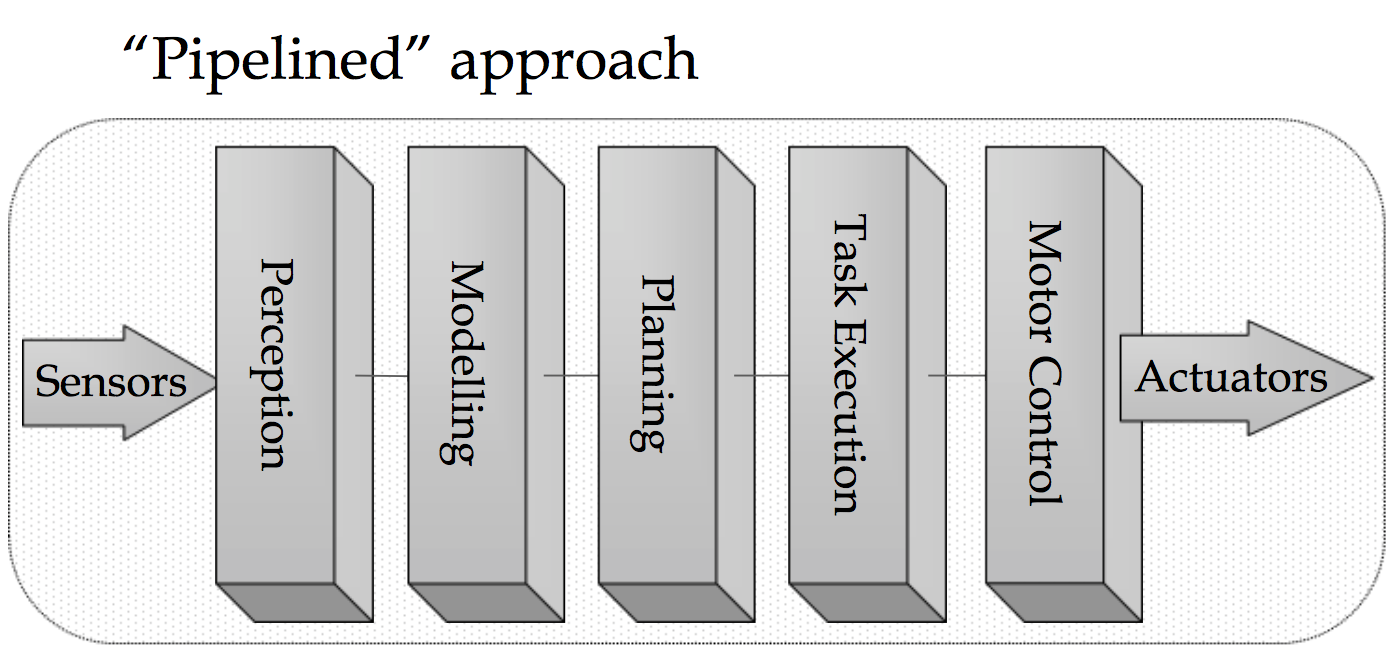
\includegraphics[width=\textwidth, height=4.1cm]{classical.png}
        \label{fig:classical}
    \end{subfigure}
    \begin{subfigure}[H]{0.475\textwidth}   
        \centering
        \caption{}
        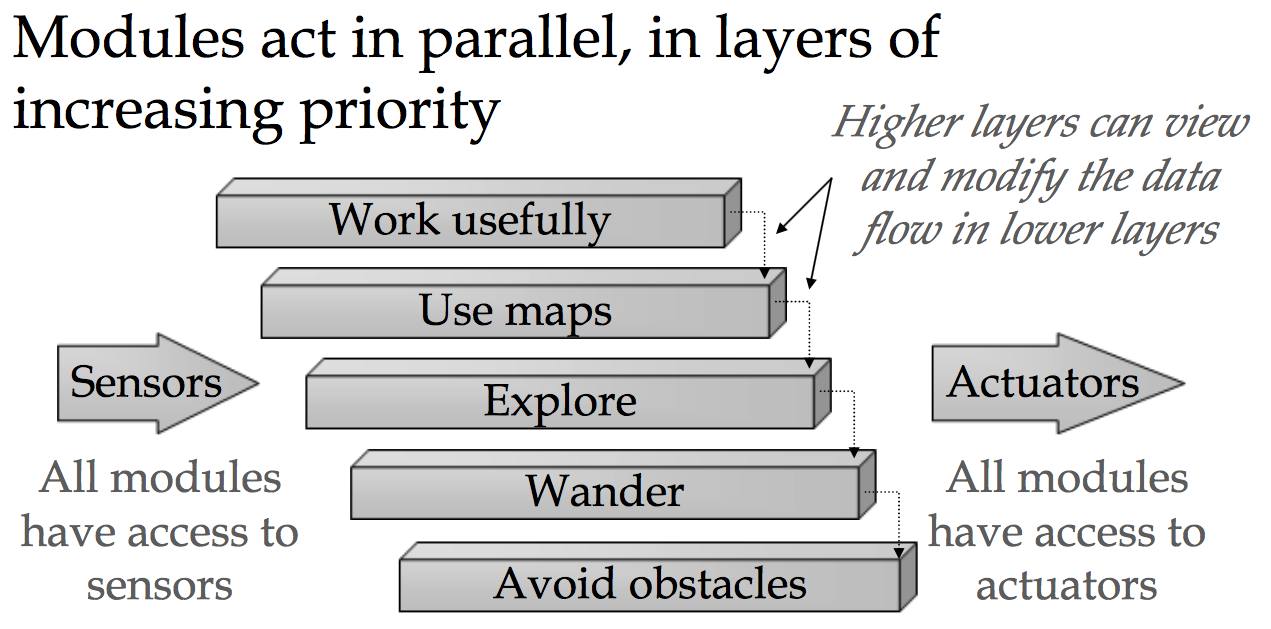
\includegraphics[width=\textwidth, height=4.1cm]{subsumption.png}
        \label{fig:subsumption}
    \end{subfigure}
    \caption{Robotic architectures: (a) Classical approach. (b) Subsumption approach.}
\end{figure}
Two main architectures exist to develop robotic behaviour have been used in multiple robotic systems: a classical approach and a subsumption architecture \cite{subsumption}. A classical architecture is based on a pipeline-like approach, where first perception occurs, building up a model of the world, then from that model, planning is made then tasks are executed, shown in \textbf{\Cref{fig:classical}}. A subsumption architecture works in more of a layered model, where multiple tasks run at the same time, so the layers act in parallel. That means that tasks such as exploration and wandering would run together, both with access to the robot's motors (shown in \textbf{\Cref{fig:subsumption}}).
\newline\newline
The simplest approach to the shopkeeper's architecture seems to be a classical pipeline approach. It doesn't make sense for a subsumption architecture, since Baxter will need to re-analyse his environment before planning any manipulation tasks. Therefore a basic logical behaviour architecture could be theorised for a simple task of picking up sweets. In an example task, Baxter would want to pick up a sweet from a pile of sweets on the table. This could be split into a logical order of behaviours: recognise the sweets on the table, plan which sweet he wants to pick up, then pick up the sweet. This has to be done in this order, as Baxter will need to build up a model of his environment before he can perform the task.
\section{Machine Vision}
Machine vision is the area of computer science where images can be analysed and understood. This is often used in robotics to help robots recognise and understand objects in their environment so they can react and respond appropriately. In the sweet shop, Many robotic vision systems are used in conjunction with manipulation and other aspect's of the robot's behaviour, so a robot will recognise and understand it's surrounding and interpret that in real-time to feed the information back to other processes. For example, this technique could be applied to Baxter looking at the table and then telling the manipulation process where a sweet is located to pick it up.
\subsection{Image Segmentation Techniques}
There have been multiple approaches to object detection in machine vision. The approaches analyse pixels by segmenting images into the desired edges/distinguishing features. The main object detection methods found in preliminary research that could be applied to sweet recognition in the project were active contour methods and template matching.
\newline\newline
There are multiple methods of active contour detection in images, all based around the principle of detecting object boundaries, iteratively moving towards the ideal border using image processing and user input \cite{activecontours, mortensen}. Contours work by assigning a general snake-like shape to roughly form a border around the target object. After, internal and external spline energies are calculated to determine where the border should be attracted to, whether it be a strong edge gradient (a defined edge on an object), a dark ridge or a termination of an edge. This energy potential is calculated using the edge, line and term terms using the formula below:
\begin{center}
$\varepsilon$\textsubscript{image} = $\omega$\textsubscript{line}$\varepsilon$\textsubscript{line} + $\omega$\textsubscript{edge}$\varepsilon$\textsubscript{edge} +  $\omega$\textsubscript{term}$\varepsilon$\textsubscript{term}
\end{center}
Here, $\varepsilon$ refers to energy, $\omega$ represents the weight of the line, edge and termination features. The contour `evolves' by using this formula to minimise the energy, which moves inwards towards a contour that perfectly outlines an object, shown by the moving `snake' contour in \textbf{\Cref{fig:snake}}. The fact that the contour energies need to be minimised means that it is helpful to initialise a contour external to the object's border. Active contour methods are commonly used in situations where a defined border exists to clearly view an object, which could come in handy when recognising sweets on a table later on.
\begin{figure}[H]
    \captionsetup[figure]{justification=centering}
    \begin{subfigure}[H]{0.475\textwidth}   
        \centering 
        \caption{}
        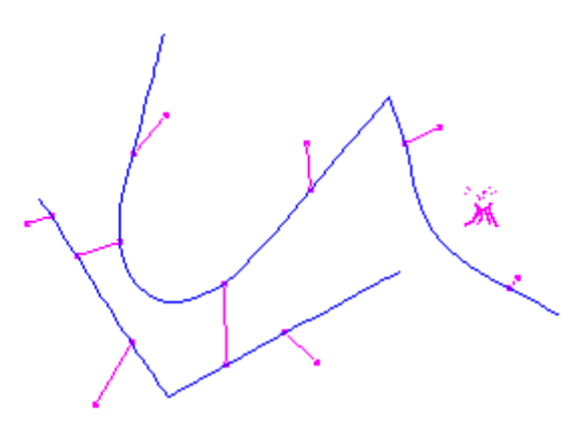
\includegraphics[width=\textwidth, height=4.1cm]{snake.png}
        \label{fig:snake}
    \end{subfigure}
    \begin{subfigure}[H]{0.475\textwidth}   
        \centering
        \caption{}
        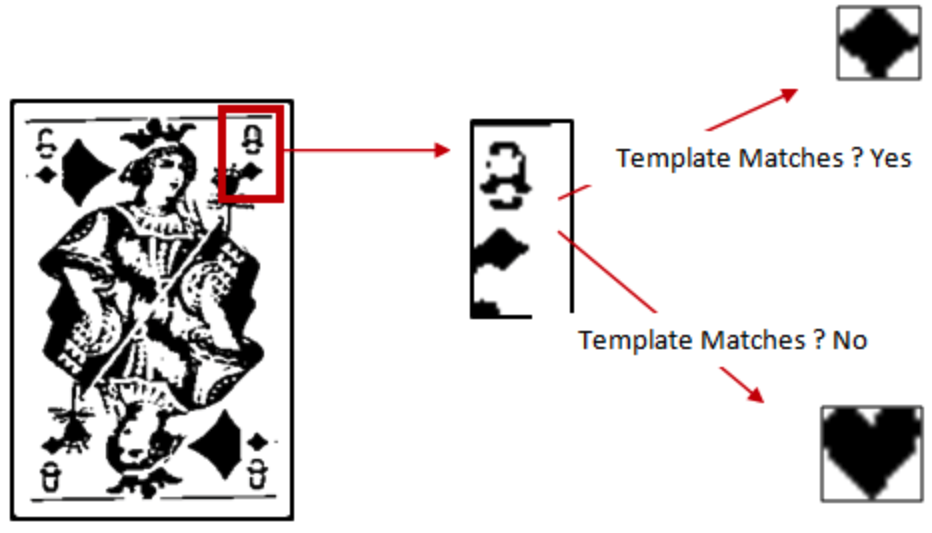
\includegraphics[width=\textwidth, height=4.1cm]{template.png}
        \label{fig:template}
    \end{subfigure}
    \captionsetup{justification=centering}
    \caption{Image processing techniques: (a) A snake contour being attracted to a dark edge. (b) An example of template matching on a playing card.}
\end{figure}
Another method which could be applied to recognising sweets is template matching, where the shape of a sweet could be learnt to recognise them in different orientations. Template matching uses an approach using the template image (for example, a picture of a sweet) and tries to match that image to an area of the target image in a particular orientation. An example of template matching is shown in \textbf{\Cref{fig:template}}, where numbers and suit template images can be detected on the playing card. The key aspects of this technique is establishing a way to measure the error metric, so the template and image can be compared. Also, a successful search technique needs to be devised to search where the template matches occur and at what rotation. A common error metric is the least squares method, where each x, y pixel is compared to an u, v position in the target image \cite{robuststats}. Search methods need to be developed appropriately too, as an exhaustive search is inefficient to search all orientations. Some solutions to this problem include limiting the space to search over, such as hierarchical motion estimation, where an image pyramid is created, searching first at more coarse levels, then each of those searches is used to initialise a more local search at the next level \cite{quam}. This method is also a viable method to search and locate sweets on a table image.
\subsection{Pointcloud Analysis}
Vision techniques used in a 3D Pointcloud have a slightly different approach. Instead of segmenting and processing the pixels in an image, object analysis is more concentrated around grouping of points that are close in orientation and colour.\newline\newline
Pointcloud's are analysed in a different way to regular 2D images. However, the same basic image processing principles still apply, segment out the area you want to analyse and use a recognition technique to provide further recognition. A main method of initially segmenting pointclouds is to use RANSAC \cite{ransac}, which can be used to find co-planar points. RANSAC (or random sample consensus), is a technique first developed as an alternative to a least median square method. To find points on a particular plane, a targeted sample of vertices from the pointcloud are analysed and checked whether they mathematically lie near enough to each other to belong to the same plane. These planes can then be used to find manmade objects within the 3D cloud, with flat, parametric surfaces. This technique is commonly used to segment objects from unwanted surfaces, for example, separating objects on top of the shop counter from the table itself. RANSAC can also be used to identify simple 3D shapes such as cylinders by searching over points that fit a mathmatical model, as shown in \textbf{\Cref{fig:objectransac}}.
\begin{figure}[H]
    \captionsetup[figure]{justification=centering}
    \begin{subfigure}[H]{0.475\textwidth}   
        \centering 
        \caption{}
        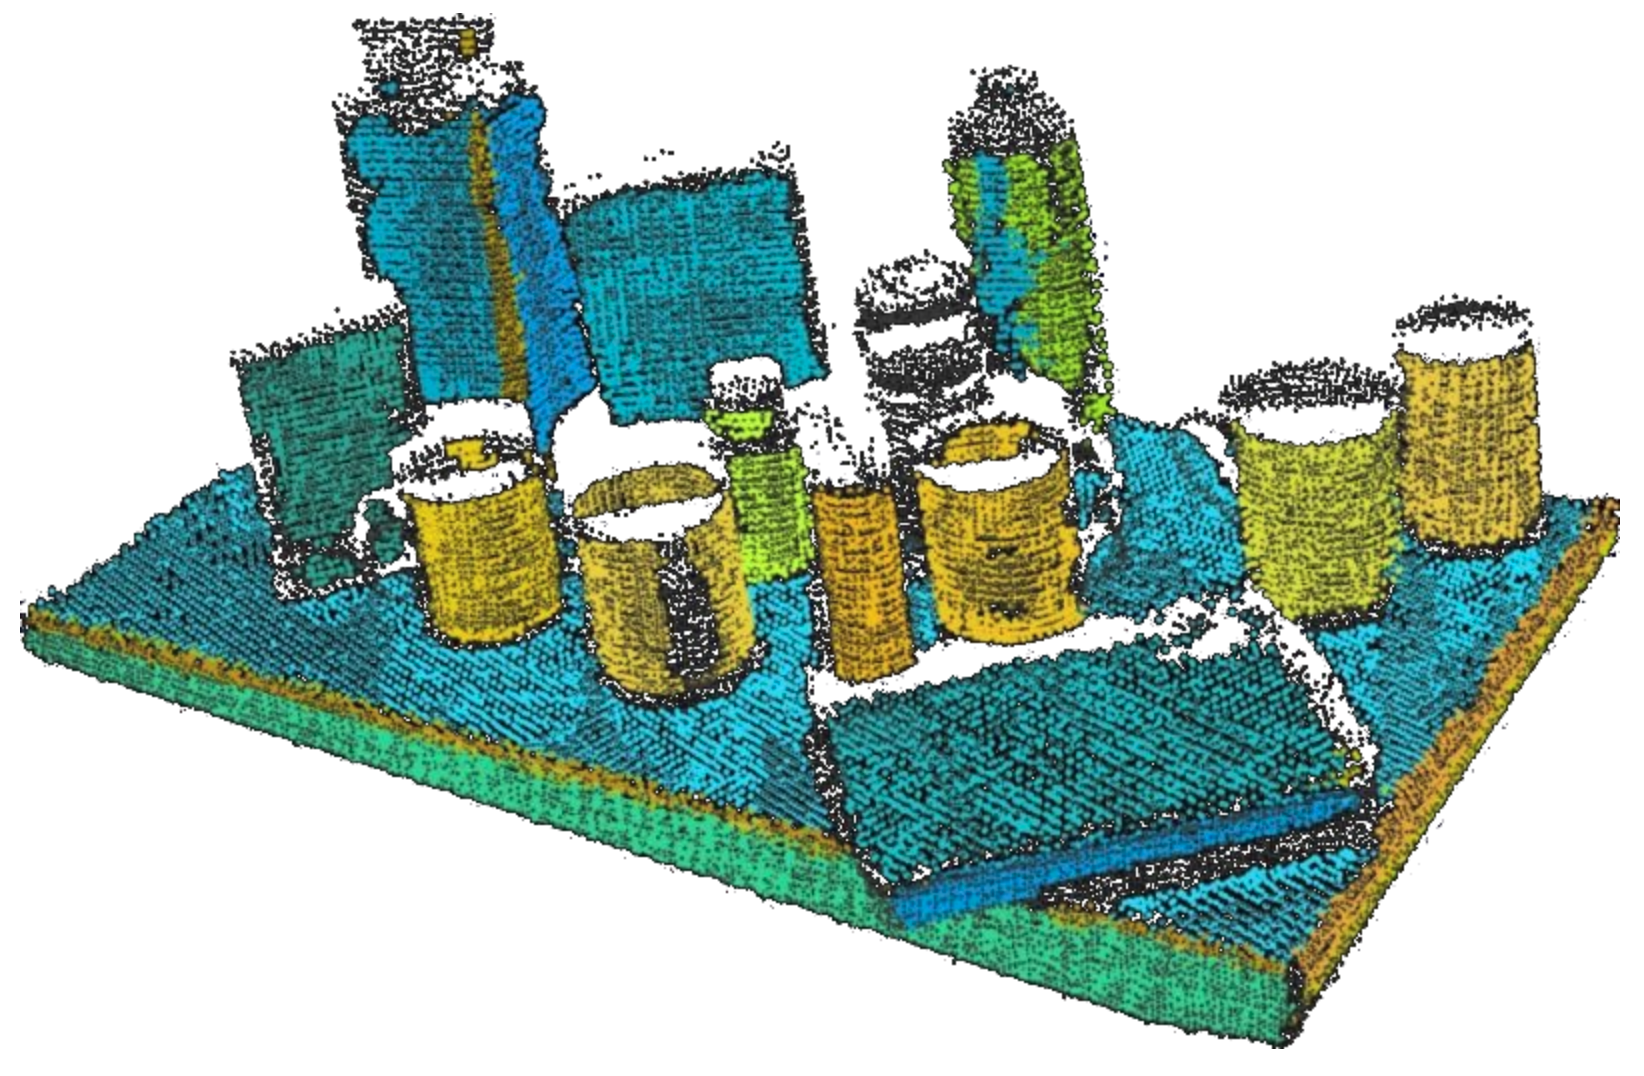
\includegraphics[width=\textwidth, height=4.3cm]{ransacobjects.png}
        \label{fig:objectransac}
    \end{subfigure}
    \begin{subfigure}[H]{0.475\textwidth}   
        \centering
        \caption{}
        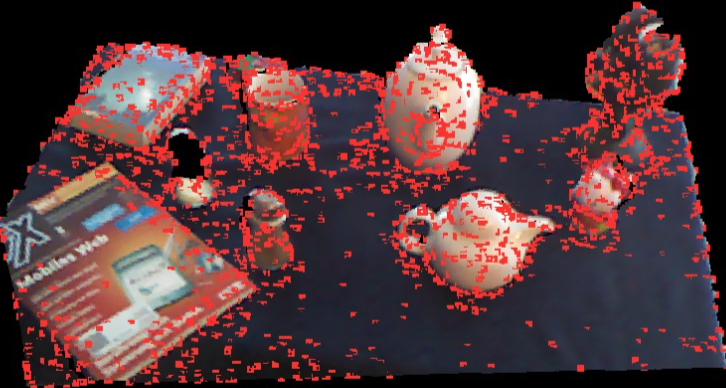
\includegraphics[width=\textwidth, height=4.3cm]{3dsift.png}
        \label{fig:3dsift}
    \end{subfigure}
    \captionsetup{justification=centering}
    \caption{Pointcloud processing techniques: (a) RANSAC detection of cylindrical objects. (b) 3D-SIFT detected keypoints in an object pointcloud.}
\end{figure}
Another method to recognise objects within a pointcloud exists as a 3D expansion similar to a template matching method, where a 3D model can be built of a target object \cite{3dmodels}. To create a single model representation of an object, multiple images can be combined into one 3-dimensional representation, allowing the object to be recognised from multiple viewpoints. Once the model has been built, SIFT (Scale Invariant Feature Transform) features can be retrieved from a 2D RGB view of the object, which can retrieve a vector of feature points invariant to translation, scaling, rotation and illumination, shown in \textbf{\Cref{fig:3dsift}}. The SIFT features can then be matched to their nearest neighbours with the closest Euclidean distances, which can then determine if that matches the target object at a specific 3D orientation. This would then mean that the object would then be recognised and at what orientation in the pointcloud. This can be used as an approach to find 3D objects on the table, such as a bowl holding the sweets.
\section{Manipulation Planning}
Manipulation planning is a key aspect of robotic systems, where the hardware of the robot and the limitations need to be considered before integrating manipulation techniques. Manipulation tasks in the sweet shop include tasks such as picking up sweets, giving them to the customer, which will all require planning for the position and movement of the grippers.
\subsection{Inverse Kinematics and Planning}
Inverse kinematics is one of the common movement planning techniques in robotics. This involves a kinematic analysis of the current state of the robot's system, looking at the all of the joint positions and angles. Forward kinematics works out where the endpoint of a manipulator is, given the angles between each limb (i.e. joint angles). Inverse kinematics does the exact reverse of this, where you specify a coordinate endpoint of the limb and the joint angles between each link will be worked out. Baxter's inverse kinematics requires a specified x, y, z coordinate for an effector's endpoint, along with a quaternion for the rotation of the arm.
\newline\newline
After the inverse kinematics calculations have been done, a planning algorithm has to be used to decide which is the best way Baxter can move his arm to the calculated joint angles. One of the main issues with planning is that commonly, there are multiple paths to take and it is not always clear which one is the best to take. The most obvious solution to choose would be to select the one which contains the least overall movement to get to the right location. The problem with the multiple solutions is that sometimes, unexpected routes can be taken instead of the desired one. This usually tends to occur because a perceived human solution to a joint position will not be the closest solution in the joint's coordinate system, rather than the world coordinate system \cite{robotintro}.
\subsection{Grasping Methods}
In the shopkeeper-customer interaction, there will be multiple parts of the interaction that require Baxter to grasp objects in different ways. One task that needs to be done is for Baxter to grasp sweets from a table. Multiple techniques could be used to do this, but a sensible approach would seem to be using a PCA (principal component analysis) to get the correct grasping angle to approach the sweet \cite{PCA}. Once the angle was obtained, Baxter could grasp the sweet from the correct angle to pick it up.
\newline\newline
Further manipulation issues could be encountered if Baxter wants to exchange money between him and the customer. This would be due to notes being soft-bodied, providing issues in separating notes and grasping them to begin with. There are multiple areas of research into soft-bodied grasping and manipulation, which is an unsolved problem in robotics as of yet as the object changes shape while being grasped. One approach to do this is done using robot towel folding using cloth grasping \cite{clothgrasp}.
\section{Planning Under Clutter}
Planning under clutter could be an important aspect of the project depending on how the sweets are placed on the table. If they were grouped together, Baxter would have to plan to separate them from the clutter. Also, other objects on the shop's counter could cause clutter issues with recognition and manipulation planning.
\newline\newline
One task that needs to be done, is for Baxter to be able to grasp and separate sweets. Separating the sweets out on the table with grasping methods could be done in multiple different ways, such as picking the sweets up and dropping them from a height onto the table \cite{clutter}, or scooping some sweets up with the gripper and looking at the sweets in Baxter's hand at that time. Multiple planning methods need to be incorporated to separated groups of sweets on the table, using a vision system that can separate the pile into graspable and non-graspable sweets.
\newline\newline
Other tasks that could involve planning under clutter could be perception tasks in clutter. With multiple items on the shop's counter, such as sweets, containers and possibly other items, the vision systems have to be accurate enough to ignore other objects and clutter and concentrate on the desired shape/size of the target object.
\section{Interacting with People}
Human interaction is key to making the robot shopkeeper a realistic and comprehensive experience. By testing with human customers, this system could be made robust and efficient. This is important for Baxter to understand the customer's request and interact with them accordingly in the shop.
\newline\newline
Voice recognition is a useful feature to integrate robot and customer interaction in the shop. Multiple techniques have been developed over time for speech recognition \cite{speech}, some of which are Python's NLTK module. Using these principles, speech can be converted to text and then analysed for commands the customer can give to Baxter.
\captionsetup[figure]{justification=centering}
\begin{figure}[H]
        \centering 
        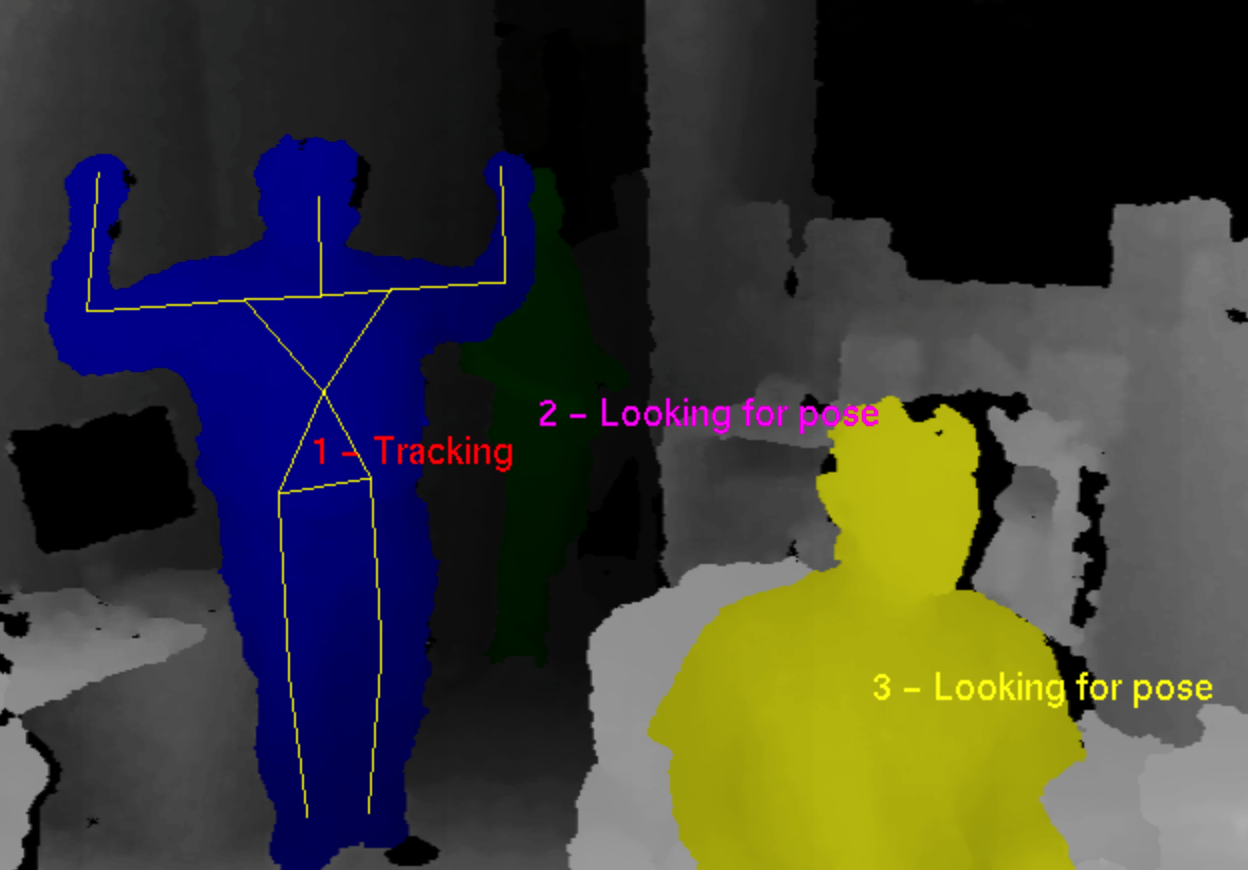
\includegraphics[width=0.5\textwidth, height=5cm]{skeletontracking.png}
        \caption{Openni\_tracker tracking skeletons and poses from a Kinect depth image.}
        \label{fig:skeletons}
\end{figure}
Another useful feature in Baxter interacting with the customer is skeleton recognition, which would allow Baxter to recognise the gestures the customer is doing, such as reaching for a bag of sweets or reaching out with some money. Different approaches have been used for skeleton recognition, but a relatively easy implementation of this is to use the Kinect's in-built skeleton recognition to detect people and their positions in front of the camera. \textbf{\Cref{fig:skeletons}} above shows an example of how simple poses and skeletons can be tracked using Openni\_tracker\footnote{ROS Wiki: Openni\_tracker. \url{http://wiki.ros.org/openni\_tracker}}. This technology could ideally be used to detect someone holding their hand out to exchange money with Baxter in the shop.